\section{Datenbankkonzept und architektonische Entscheidungen}
\setauthor{Markus Tran}

Für das Backend der Anwendung spielt die Wahl der geeigneten Datenbanktechnologie
eine zentrale Rolle. Trotz vorhandener Kenntnisse im Bereich nicht-relationaler
Datenbanken (NoSQL) -- wie etwa MongoDB oder Vektordatenbanken -- wurde im Rahmen
dieses Projekts bewusst eine relationale Datenbank eingesetzt.

Die Entscheidung für ein relationales Datenbanksystem basiert auf mehreren Faktoren.
Die Anwendung weist eine klar strukturierte und logisch getrennte Datenarchitektur
auf, wodurch sich die Daten und deren Beziehungen gut in einem relationalen Modell
abbilden lassen. Entitäten und ihre Relationen konnten somit eindeutig definiert
und konsistent strukturiert werden. Dieses Vorgehen entspricht dem etablierten
Standard bei Anwendungen mit stark strukturierten Daten und klar definierten
Geschäftsprozessen.

Ein weiterer wesentlicher Aspekt ist die Skalierbarkeit des Projekts. Relationale
Datenbanken bieten durch Normalisierung, Transaktionssicherheit (ACID-Prinzip) und
klar definierte Beziehungen eine stabile Grundlage für zukünftige Erweiterungen.
Voraussetzung für eine nachhaltige Skalierbarkeit ist jedoch eine sorgfältig
durchdachte Datenbankstruktur. Eine frühzeitig geplante und konsistente Modellierung
-- beispielsweise durch ein Entity-Relationship-Diagramm (ERD) -- ist essenziell,
um spätere strukturelle Anpassungen zu minimieren.


\begin{figure}[h]
    \centering
    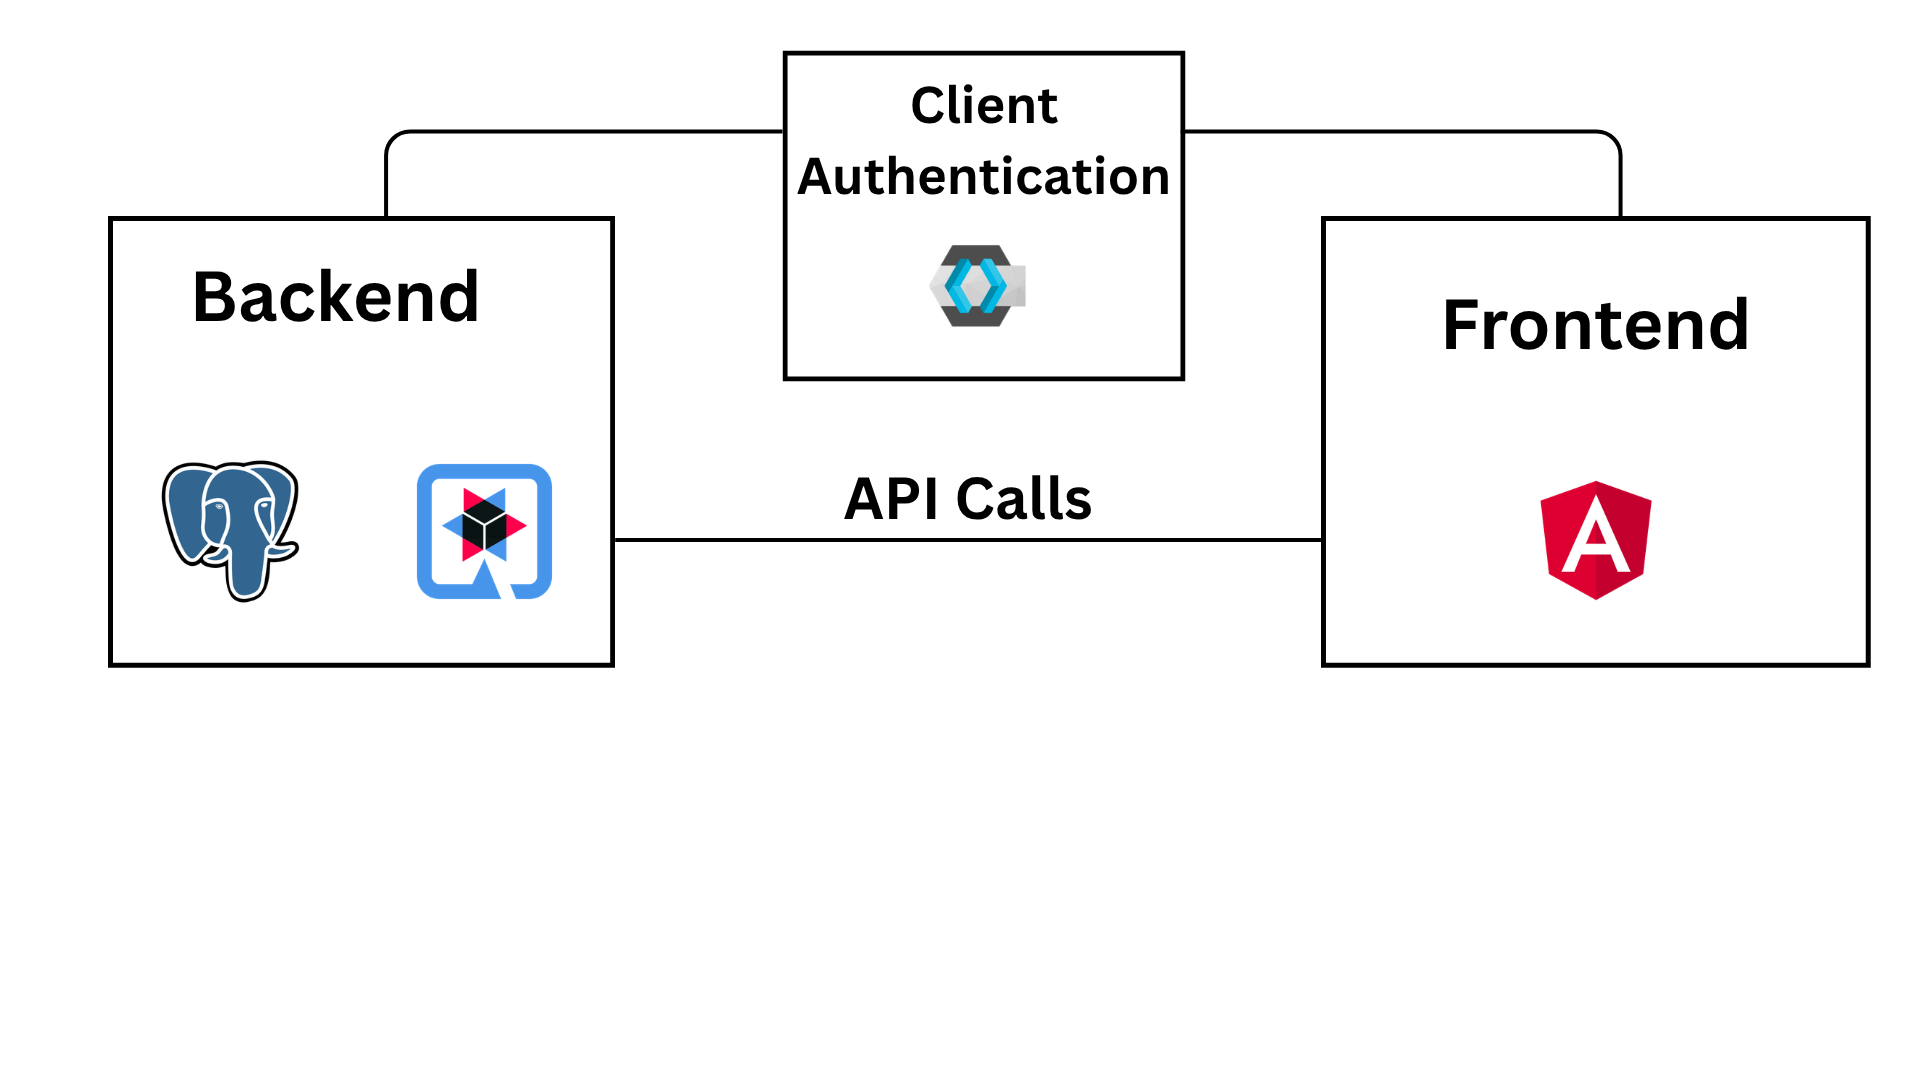
\includegraphics[width=1\textwidth, height=0.8\textheight, keepaspectratio]{pics/Architecture.png}
    \caption{Erstes Entity-Relationship-Diagramm der Anwendung}
    \label{fig:erd_v1}
\end{figure}



\subsection{Herausforderungen im Entwicklungsprozess}

Im Verlauf der Diplomarbeit traten mehrere strukturelle Herausforderungen auf, die
im Sinne einer transparenten Dokumentation offen dargestellt werden sollen.

Zu Beginn der Implementierungsphase wurde ohne vollständig ausgearbeitetes
Gesamtkonzept mit der Programmierung begonnen. Das Entity-Relationship-Diagramm
wurde parallel zur Entwicklung erstellt, wodurch sich die Datenbankstruktur
dynamisch entwickelte. Dieses iterative Vorgehen führte zwar zu schneller
praktischer Umsetzung, hatte jedoch den Nachteil, dass strukturelle Änderungen
im Nachhinein größeren Anpassungsaufwand verursachten.

\begin{figure}[h]
    \centering
    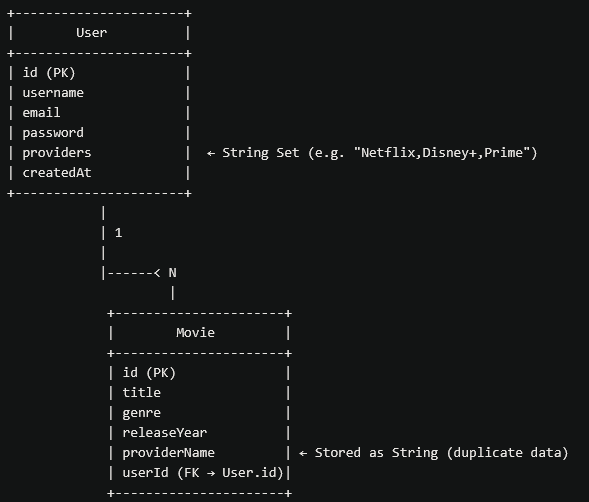
\includegraphics[width=0.9\textwidth]{pics/erd_v1}
    \caption{Erstes Entity-Relationship-Diagramm der Anwendung}
    \label{fig:erd_v1}
\end{figure}

Eine weitere wesentliche Herausforderung ergab sich durch die späte Integration
von Keycloak als Identity- und Access-Management-Lösung. Ursprünglich war die
Benutzerverwaltung eigenständig implementiert worden. Durch die nachträgliche
Einführung von Keycloak mussten die bestehenden User-Strukturen grundlegend
überarbeitet werden. Dies hatte zur Folge, dass die Benutzerentitäten angepasst
werden mussten, die Authentifizierungs- und Autorisierungslogik neu strukturiert
wurde sowie abhängige Klassen und Beziehungen refaktoriert und teilweise neu
implementiert werden mussten. Diese Umstellung führte zu zusätzlichem
Entwicklungsaufwand, zeigte jedoch zugleich die Bedeutung einer frühzeitigen
Architekturentscheidung -- insbesondere im Bereich der Sicherheits- und
Authentifizierungsmechanismen.

\begin{figure}[h]
    \centering
    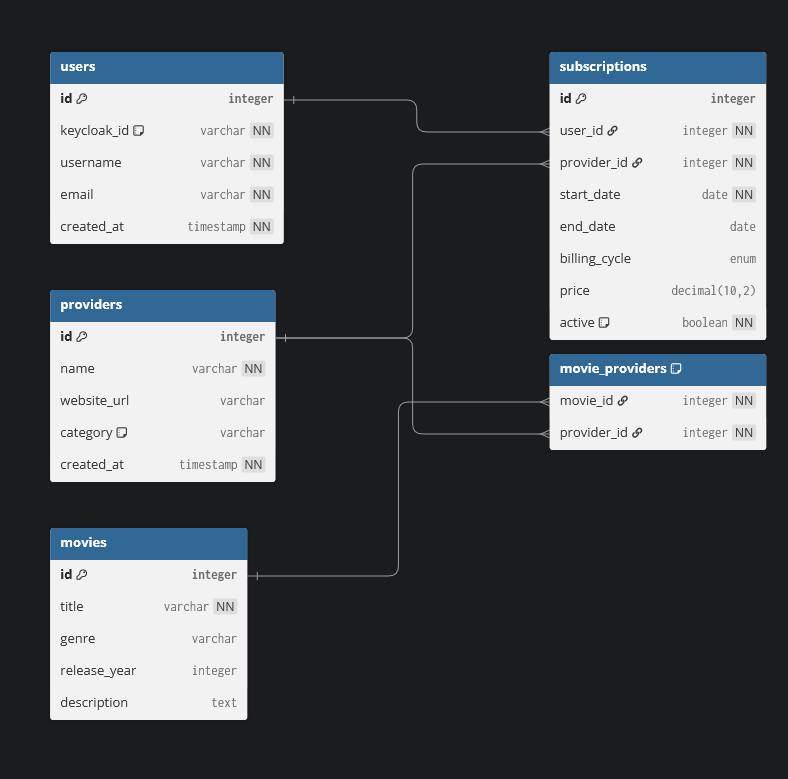
\includegraphics[width=0.9\textwidth]{pics/erd_v2}
    \caption{Überarbeitetes Entity-Relationship-Diagramm nach Integration von Keycloak}
    \label{fig:erd_v2}
\end{figure}


\subsection{Modellierung der Many-to-Many-Beziehung und strukturelle Weiterentwicklung}

Im weiteren Verlauf der Systemarchitektur zeigte sich deutlich der Mehrwert einer
sauberen relationalen Modellierung, insbesondere bei der Abbildung von
Many-to-Many-Beziehungen.

Im Kontext der vorliegenden Applikation -- einem Mediatheken-Abonnement-Manager --
besteht zwischen den Entitäten \textit{User} und \textit{Provider} keine einfache
1:n-Beziehung, sondern eine n:m-Beziehung. Ein Benutzer kann mehrere Anbieter
abonnieren, während ein Anbieter von mehreren Benutzern genutzt werden kann.

Die Einführung einer eigenständigen Relationstabelle (\texttt{UserProviderSubscription})
dient hierbei nicht ausschließlich der technischen Verknüpfung zweier Fremdschlüssel.
Vielmehr übernimmt diese Tabelle eine fachlich zentrale Rolle innerhalb des
Domänenmodells. In der Relationstabelle werden zusätzliche Attribute gespeichert,
die die konkrete Ausprägung der Beziehung beschreiben:

\begin{itemize}
    \item Beginn des Abonnements (Startdatum)
    \item Ende des Abonnements (Enddatum)
    \item Zahlungszyklus (Enum: monatlich oder jährlich)
\end{itemize}

Diese Attribute gehören semantisch weder ausschließlich zum Benutzer noch
ausschließlich zum Anbieter, sondern definieren die konkrete Vertragsbeziehung
zwischen beiden Entitäten. Die Modellierung über eine separate Relationstabelle
ermöglicht somit eine fachlich korrekte Abbildung der Geschäftslogik, die
Erweiterbarkeit um weitere beziehungsbezogene Attribute -- etwa Preis, Rabatt
oder Kündigungsstatus -- sowie eine klare Trennung der Verantwortlichkeiten
innerhalb des Datenmodells. Gerade an dieser Stelle wird deutlich, dass
relationale Datenbanken ihre Stärke bei strukturierten und stark
beziehungsorientierten Datenmodellen ausspielen.

\subsection{Reflexion der anfänglichen Modellierungsentscheidung}

Rückblickend stellt sich die anfängliche Entscheidung, Anbieter als
\texttt{Set<String>} direkt innerhalb der User-Entität zu speichern, als
struktureller Fehler heraus. Diese vereinfachte Modellierung war zwar für einen
ersten Prototyp funktional ausreichend, führte jedoch zu mehreren konzeptionellen
Einschränkungen:

\begin{enumerate}
    \item Es konnten keine anbieterspezifischen Metadaten gespeichert werden
    (z.\,B. Website, Kategorie oder Beschreibung).
    \item Die konkrete Ausgestaltung der Beziehung -- Startdatum, Zahlungszyklus
    etc. -- war nicht modellierbar.
    \item Eine konsistente Datenhaltung war nicht gewährleistet, da String-Werte
    fehleranfällig und nicht referenziell abgesichert sind.
    \item Erweiterungen des Systems hätten tiefgreifende strukturelle Änderungen
    erfordert.
\end{enumerate}

Insbesondere der Umstand, dass beziehungsrelevante Informationen nicht abgebildet
werden konnten, verdeutlicht die Problematik dieser frühen Designentscheidung.
Die Speicherung als String-Set widersprach den Grundprinzipien der Normalisierung
und verhinderte eine skalierbare Weiterentwicklung des Systems. Erst durch die
Einführung einer eigenständigen \texttt{Provider}-Entität sowie einer
Relationstabelle konnte das Datenmodell den fachlichen Anforderungen der
Applikation gerecht werden. Diese Umstrukturierung stellt einen wesentlichen
architektonischen Reifeprozess im Projektverlauf dar.
